%%%%%%%%%%%%%%%%%%%%%%%%%%%%%%%%%%%%%%%%%
% Beamer Presentation
% LaTeX Template
% Version 1.0 (10/11/12)
%
% This template has been downloaded from:
% http://www.LaTeXTemplates.com
%
% License:
% CC BY-NC-SA 3.0 (http://creativecommons.org/licenses/by-nc-sa/3.0/)
%
%%%%%%%%%%%%%%%%%%%%%%%%%%%%%%%%%%%%%%%%%

%----------------------------------------------------------------------------------------
%	PACKAGES AND THEMES
%----------------------------------------------------------------------------------------

\documentclass[usenames,dvipsnames]{beamer}

\mode<presentation> {

% The Beamer class comes with a number of default slide themes
% which change the colors and layouts of slides. Below this is a list
% of all the themes, uncomment each in turn to see what they look like.

%\usetheme{default}
% \usetheme{AnnArbor}
%\usetheme{Antibes}
%\usetheme{Bergen}
% \usetheme{Berkeley}
% \usetheme{Berlin}
%\usetheme{Boadilla}
%\usetheme{CambridgeUS}
% \usetheme{Copenhagen}
\usetheme{Darmstadt}
% \usetheme{Dresden}
% \usetheme{Frankfurt}
% \usetheme{Goettingen}
%\usetheme{Hannover}
%\usetheme{Ilmenau}
%\usetheme{JuanLesPins}
%\usetheme{Luebeck}
% \usetheme{Madrid}
% \usetheme{Malmoe}
%\usetheme{Marburg}
% \usetheme{Montpellier}
% \usetheme{PaloAlto}
% \usetheme{Pittsburgh}
%\usetheme{Rochester}
% \usetheme{Singapore}
%\usetheme{Szeged}
%\usetheme{Warsaw}

% As well as themes, the Beamer class has a number of color themes
% for any slide theme. Uncomment each of these in turn to see how it
% changes the colors of your current slide theme.

% \usecolortheme{albatross}
%\usecolortheme{beaver}
%\usecolortheme{beetle}
%\usecolortheme{crane}
%\usecolortheme{dolphin}
%\usecolortheme{dove}
%\usecolortheme{fly}
\usecolortheme{lily}
%\usecolortheme{orchid}
%\usecolortheme{rose}
%\usecolortheme{seagull}
%\usecolortheme{seahorse}
%\usecolortheme{whale}
%\usecolortheme{wolverine}

%\setbeamertemplate{footline} % To remove the footer line in all slides uncomment this line
%\setbeamertemplate{footline}[page number] % To replace the footer line in all slides with a simple slide count uncomment this line

%\setbeamertemplate{navigation symbols}{} % To remove the navigation symbols from the bottom of all slides uncomment this line
}

% % -------------------------------------------
% % Songkai added, feel free to delete --------
% \AtBeginSection[]{
%   \begin{frame}
%   \vfill
%   \centering
%   \begin{beamercolorbox}[sep=8pt,center,shadow=false,rounded=true]{title}
%     \usebeamerfont{title}\insertsectionhead\par%
%   \end{beamercolorbox}
%   \vfill
%   \end{frame}
% }
% % Songkai added, feel free to delete --------
% % -------------------------------------------

\usepackage{graphicx} % Allows including images
\usepackage{booktabs} % Allows the use of \toprule, \midrule and \bottomrule in tables
\usepackage{natbib}
\usepackage{xcolor}
\usepackage{amsmath, amssymb, graphicx, url}
\usepackage[ruled]{algorithm2e}
\usepackage{commath}
\usefonttheme[onlymath]{serif}

% \usepackage{amsmath}
% \usepackage{amssymb}
%\usepackage[a4paper, margin=0.8in]{geometry}
\usepackage{parskip}
% \usepackage{graphicx}

% \usepackage{natbib}
% \usepackage[colorlinks=true, linkcolor={blue}]{hyperref}

\hypersetup{pdfauthor={Name},colorlinks=true, linkcolor={white}, citecolor={teal}}

\usepackage{tabularx}
\usepackage{array}
\usepackage{makecell}
\usepackage{mathtools}
\usepackage{bm,upgreek}
\usepackage{bbm}
\usepackage{dsfont}
\usepackage{textpos}
% \usepackage{eso-pic}

\def\E{\mathbf{E}}
\def\PP{\mathbf{P}}
\def\Reals{\mathbb{R}}
\def\Naturals{\mathbb{N}}
\def\argmin{\operatornamewithlimits{arg\,min}}
\def\deq{:=}
\def\wh#1{\widehat{#1}}
\def\bd#1{\mathbf{#1}}
\def\bx{\bd{x}}
\def\by{\bd{y}}
\def\bZ{\bd{Z}}
\def\bB{\bd{B}}
\def\bV{\bd{V}}
\def\tO{{\tilde{\cO}}}
\def\tOm{\tilde{\Omega}}
\def\barw{\overline{w}}
\def\d{{\mathrm d}}
\def\ave#1{\langle #1 \rangle}
\def\Ave#1{\left\langle #1 \right\rangle}
\def\eps{\varepsilon}
\def\tr{\mathrm{Tr}}


\def\HS{\mathbb{H}}
\def\reals{\mathbb{R}}
\def\ths{\theta^*}
\def\thh{\hat{\theta}}
\def\lbr{\left[}
\def\rbr{\right]}
\def\lc{\left(}
\def\rc{\right)}


    \def\ddefloop#1{\ifx\ddefloop#1\else\ddef{#1}\expandafter\ddefloop\fi}
    % \cA, \cB, ...
    \def\ddef#1{\expandafter\def\csname c#1\endcsname{\ensuremath{\mathcal{#1}}}}
    \ddefloop ABCDEFGHIJKLMNOPQRSTUVWXYZ\ddefloop
    \def\argmin{\operatornamewithlimits{arg\,min}}
    \def\E{\mathbf{E}}
    \def\bx{\bd{x}}
	\def\by{\bd{y}}
    \def\bZ{\bd{Z}}

\newcommand{\propnumber}{} % initialize
\newtheorem*{prop}{Proposition \propnumber}
\newenvironment{propc}[1]
  {\renewcommand{\propnumber}{#1}%
   \begin{shaded}\begin{prop}}
  {\end{prop}\end{shaded}}

\newcommand{\crlrnumber}{} % initialize
%\newtheorem*{corollary}{Corollary \crlrnumber}
\newenvironment{corollaryc}[1]
  {\renewcommand{\crlrnumber}{#1}%
   \begin{shaded}\begin{corollary}}
  {\end{corollary}\end{shaded}}

\theoremstyle{definition}
% \newtheorem{definition}




% \setbeamertemplate{headline}{% 
%     \leavevmode%
%     \hbox{%
%         \begin{beamercolorbox}[wd=.4\paperwidth,ht=2.25ex,dp=1ex,right]{section in head/foot}%
%             \usebeamerfont{section in head/foot}\insertshorttitle\hspace*{2ex}
%         \end{beamercolorbox}%
%         \begin{beamercolorbox}[wd=.6\paperwidth,ht=2.25ex,dp=1ex,left]{subsection in head/foot}%
%             \usebeamerfont{section in head/foot}
\includegraphics[height=2ex,keepaspectratio]{Slides/Block_M-Hex.png}\hspace*{2ex}\insertsectionhead
%         \end{beamercolorbox}%
%     }
% }

% \addtobeamertemplate{headline}{}{%
% \begin{textblock*}{100mm}(.85\textwidth,-1cm)
% \Huge\textcolor{white}{\textbf{\TeX}}
% \end{textblock*}}



%----------------------------------------------------------------------------------------
%	TITLE PAGE
%----------------------------------------------------------------------------------------

%%%% TRY WITH TEXTPOS
% \newcommand{\imgblock}{\begin{textblock*}{5cm}(10.5cm,-1.2cm) % {block width} (coords)
%         
\includegraphics[width=1cm]{Slides/Block_M-Hex.png} % loading the image
%     \end{textblock*}
%     }

% \addtobeamertemplate{background}{\imgblock}{}



% \setbeamertemplate{headline}{\hfill
\includegraphics[width=1.5cm]{Slides/Block_M-Hex.png}\hspace{0.2cm}\vspace{-1cm}}

% \logo{
\includegraphics[height=1cm]{Slides/Block_M-Hex.png}}

\addtobeamertemplate{frametitle}{}{%
    \begin{textblock*}{5cm}(10.5cm, -0.8cm)
        
\includegraphics[width=0.9cm]{Slides/Block_M-Hex.png} % your logo file here
    \end{textblock*}
}

\usepackage{xcolor}
\definecolor{mycolor}{cmyk}{100, 60, 0, 60}


% \setbeamertemplate{footline}[text line]{%
%   \parbox{\linewidth}{\vspace*{-8pt}some text\hfill\insertshortauthor\hfill\insertshorttitle\hfill\insertshortinstitute}}
% \setbeamertemplate{navigation symbols}{}

\setbeamercolor{frametitle}{bg=mycolor}

\title[Journal Club]{Reading Group: Neural Operators} % The short title appears at the bottom of every slide, the full title is only on the title page

% \author[Aniket Jivani]{Aniket Jivani}
% \institute[U-M]{University of Michigan}

\date{\today}

% \AtBeginSection[]
% {
%  \begin{frame}<beamer>
%  \frametitle{Plan}
%  \tableofcontents[currentsection]
%  \end{frame}
% }

\begin{document}

\begin{frame}
\titlepage % Print the title page as the first slide
\end{frame}

% \frame{\tableofcontents}

% \begin{frame}
%  % \frametitle{Overview} % Table of contents slide, comment this block out to remove it
%  \tableofcontents % Throughout your presentation, if you choose to use \section{} and \subsection{} commands, these will automatically be printed on this slide as an overview of your presentation
% \end{frame}

\section{Introduction}
\begin{frame}{TLDR}
    Reference: \cite{Kovachki2023}, \cite{li_fourier_2021}

    TLDR: \emph{Discretization invariant methods} for solving differential equations. 4 design choices for implementing neural operators, comparisons to other methods on different PDE examples, extensions to special cases.
\end{frame}

\begin{frame}{Definition}
    \begin{enumerate}
        \item Works on any discretization or set of points in the input domain 

        \item Can be evaluated at any point of output domain i.e. apply to data given at any resolution on any mesh.

        \item Converges to Continuum operator as discretization is refined (though method itself is black-box without knowledge of underlying PDE)
    \end{enumerate}
\end{frame}

\begin{frame}{Other methods}

    I feel this is not clearly explained in the paper, and I don't think its apples-to-apples comparison.
    \begin{enumerate}
        \item Mostly defined on fixed grids, require interpolation of solution to other resolutions.

        \item \textcolor{red}{if normalized by grid size, CNNs, can be applied to uniform grids with different resolutions, 
        $\cdots$ are not universal approximators of operators.}

        \item PINNs are pointwise NNs $\implies$ discretization invariant, however, \textcolor{red}{only represent solution function of one instance.}
    \end{enumerate}
\end{frame}

\begin{frame}{Notation - part 1}
    $$\begin{aligned}(\mathsf L_au)(x)&=f(x),\quad&x\in D,\\u(x)&=u_0(x),\quad&x\in\partial D\end{aligned}$$

    $a \in \mathcal{A}: $ underlying parameter, $\mathbb{R}^{d_a}$
    
    $D \subset \mathbb{R}^d$: domain for $x$
    
    $u \in \mathcal{U}: D \rightarrow \mathbb{R}$: solution

    Recover $\mathcal{G}^{\dagger}:=\mathsf{L}_{a}^{-1}f:\mathcal{A}\rightarrow\mathcal{U}$ given pairs $\{a^{(i)}, u^{(i)}\}_{i=1}^{N}$, $a^{(i)}$ i.i.d. from measure $\mu$ \textcolor{red}{}

    approximate by: $\mathcal{G}_{\theta}:\mathcal{A}\rightarrow\mathcal{U},\quad\theta\in\mathbb{R}^{p}$

     Loss: $\min_{\theta\in\mathbb{R}^{P}} \mathcal{L}_{\theta} =\min_{\theta\in\mathbb{R}^{P}}\frac{1}{N}\sum_{i=1}^{N}\|u^{(i)}-\mathcal{G}_{\theta}(a^{(i)})\|_{\mathcal{U}}^{2}$

    For proposed $\mathcal{G}_{\theta}$ and desired $\varepsilon$, $\exists p \in \mathbb{N}$ and $\theta^{\dagger} \in \mathbb{R}^{p}$ s.t. $\mathcal{L}_{\theta} < \varepsilon$
\end{frame}

\section{Methodology}
\begin{frame}{Neural Operators}
I got rid of the notation for hidden layer dimensions and assume all map to $n$ dimensional vectors, as well as $u^{(i)} \in \mathbb{R}$. This is  based on vanilla GNO method.

\begin{enumerate}
    \item \textbf{Preprocessing}: One example is to include the spatial location along with $a$ i.e. $a^{\dagger} = (x^{(i)}, a^{(i)}) \in \mathbb{R}^{(d + d_a)}$ but any and all relevant features can be supplied

    \item \textbf{Lifting} $v_0 \in \mathbb{R}^{n} = \mathcal{P}a^{\dagger}$ where $\mathcal{P} \in \mathbb{R}^{n \times (d + d_a)}$

    \item \textbf{Kernel Integration} ($t = 0, \cdots T - 1$ is layer index not time :) 
    $$v_{t + 1} \in  \mathbb{R}^n = \sigma \left(W_{t}v_t(x) + \mathcal{K}_t(v_t) + b(x)\right)$$

    \item \textbf{Projection} $u^{(i)}(x) = \mathcal{Q} v_T(x)$, $\mathcal{Q} \in \mathbb{R}^{1 \times n}$
\end{enumerate}
\end{frame}

% \begin{frame}{Crude sketch}
    
% \end{frame}

\begin{frame}{Details}
    % All differences are related to definition of kernel operator.
    % \frac{1}{|N(x)|}\Sigma_{y \in N(x)} \mathcal{K}_t (x, y) v_t
\end{frame}

\begin{frame}{Details}
    
\end{frame}

\begin{frame}{Details}
    
\end{frame}

\begin{frame}{GNO}
    
\end{frame}


\begin{frame}{FNO}
    Closely related to: feature maps for kernels : \url{https://xavierbourretsicotte.github.io/Kernel_feature_map.html}, \url{https://web.mit.edu/modernml/course/lectures/MLClassLecture3.pdf}, and development of random feature maps \url{https://arxiv.org/pdf/1610.09072.pdf}

    Also see paper by Nelsen and Stuart: \url{https://arxiv.org/pdf/2005.10224.pdf}
\end{frame}

\section{Results}
\begin{frame}{Example 1}
    
\end{frame}

\begin{frame}{Example 2}
    
\end{frame}

\begin{frame}{Comparison of architectures}
    
\end{frame}

\begin{frame}{Comparisons to strawmen}
    \begin{columns}
    \begin{column}{0.56\textwidth}
    \begin{itemize}
        \item Pointwise feedforward NNs

        \item Fully Convolutional Networks \cite{Zhu2018}

        \item PCA + NN and RBM?

        \item DeepONets
    \end{itemize}

    Problematic:
    
    \begin{itemize}
        \item PINNs instead of regular NNs, AEs instead of PCA, ODENets? evaluated at the same grid resolution.

        \item Error vs Finite Volume and spectral methods using SOTA solvers?

        \item Claimed speed-ups (up to 3 orders of magnitude faster)- where's the work-profile results?
    \end{itemize}
    \end{column}

    \begin{column}{0.48\textwidth}
        \begin{figure}
            \centering
            
\includegraphics[width=0.6\linewidth]{Slides/strawman.jpg}
            \caption{Strawman. Credit: Dall-E 3}
            \label{fig:strawmen}
        \end{figure}

        \begin{figure}
            \centering
            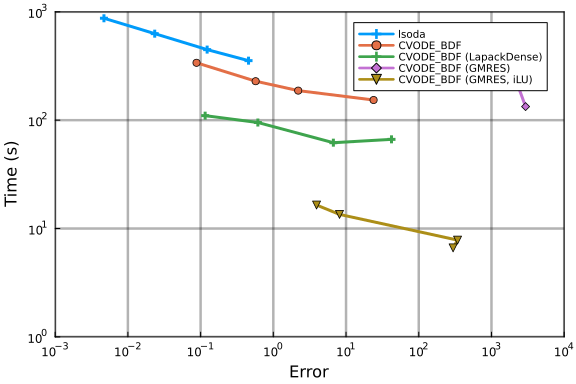
\includegraphics[width=0.5\linewidth]{Slides/work-precision.png}
            \caption{work-precision diagram. Credit: SciML benchmarks}
            \label{fig:strawmen}
        \end{figure}
        
    \end{column}
        
    \end{columns}
    
\end{frame}

\begin{frame}{DeepONet Connection}
    
\end{frame}

\section{Wrapping up}
\begin{frame}{Other interesting work}
    \begin{enumerate}
        \item PDEBench: \url{https://arxiv.org/pdf/2210.07182.pdf}

        \item Multiscale GNN Autoencoders \url{https://arxiv.org/pdf/2302.06186}
    \end{enumerate}
\end{frame}

\section{Backup}
\begin{frame}{PINNs}
    Reference: \cite{Raissi2019}

    $$f = u_t+\mathcal{N}[u]$$
    $$MSE=MSE_u+MSE_f$$

    Loss on output QoI
    $$MSE_u=\frac{1}{N_u}\sum_{i=1}^{N_u}|u(t_u^i,x_u^i)-u^i|^2$$

    Structural loss
    $$MSE_f=\frac{1}{N_f}\sum_{i=1}^{N_f}|f(t_f^i,x_f^i)|^2$$
\end{frame}

\begin{frame}{References}
\bibliographystyle{chicago}

%\bibliographystyle{IEEEtran}
\bibliography{myReference}
    
\end{frame}



\begin{frame}{}
\begin{center}
    \Large{Thank you!}
\end{center}
    
\end{frame}


\end{document}